%%%%  Las secciones de texto con fórmulas se separan con %%%%
%% Las fórmulas presentes entre 2 secciones de texto se separan con %%

%%%%%%%%%%%%%%%
%%  Capítulo 1: Introducción  %%
%%%%%%%%%%%%%%%

%%%%
\section{Reseña histórica}
\label{sec_intro_resenia}
%%%%

%%%%
Las bases de la teoría electromagnética clásica para el dominio macroscópico fueron formuladas por James Clerk Maxwell en 1873, en base al conocimiento previo desarrollado por Gauss, Ampère y Faraday, entre otros. Entre 1885 y 1887, Oliver Heaviside simplificó las expresiones e introdujo la notación vectorial actual, facilitando así el modelado de guías de ondas y líneas de transmisión \cite{Pozar:MwEngineering}.

En base a estos trabajos, Heinrich Hertz diseñó, entre 1887 y 1891, una serie de experimentos que validaron la teoría de ondas electromagnéticas propuesta por Maxwell. En 1886, Hertz construyó la primer antena dipolo, y en 1888, la primer antena parabólica, alimentada por un dipolo de 450 MHz, dando el puntapié inicial para el desarrollo de la radio durante la primera mitad del siglo \textsc{XX}.

El primer análisis de la propagación de ondas electromagnéticas en guías de ondas metálicas, publicado por Lord Rayleigh en 1897, y el posterior estudio teórico del comportamiento de ondas en guías dieléctricas por Debye y Hondros, en 1910, sentaron los cimientos para que durante la década del '30 comenzaran trabajos experimentales en transporte de ondas electromagnéticas en los laboratorios Bell \cite{Collin:GuidedWaves}.

Los conjuntos de antenas se popularizaron a partir de la aparición de la antena de Yagui-Uda en 1926, formada por elementos lineales que dan lugar a una fase fija. Recién durante la Segunda Guerra Mundial surgieron los conjuntos de antena de fase variable \cite{Stutzman:AntennaTheory}, y las guías de ondas y las antenas tomaron un lugar prioritario entre los ingenieros, matemáticos y físicos de la época, lo que permitió el desarrollo de métodos de análisis para facilitar la formulación de problemas con condiciones de borde complejas.

Recién finalizada la Segunda Guerra Mundial se comenzaron a fabricar circuitos \textit{microstrip}. En 1953, G. A. Deschamps presentó el primer trabajo sobre antenas con la misma tecnología, y la primer patente en ese sentido se registró en 1955 \cite{Balanis:Handbook}. Aún así, recién en la década del '70 comenzaron a utilizarse en aplicaciones prácticas, principalmente debido a la aparición de sustratos con bajas tangentes de pérdida, la mejora en técnicas de fotolitografía, y la optimización de modelos teóricos \cite{Barthia:Handbook}. Sin embargo, la simplificación constructiva trajo aparejados problemas de acoplamiento mutuo, que debieron ser abordados por técnicas de filtrado y blindaje.

%%%%
% NO QUEDÓ BIEN COMPLETO.
%%%%
\section{Ecuaciones de Maxwell}
\label{subsec_ecuaciones_maxwell}
%%%%
La teoría electromagnética propuesta por Maxwell, y simplificada por Heaviside, se reduce a cuatro ecuaciones diferenciales lineales vectoriales e interdependientes que, en notación diferencial, quedan expresadas de la siguiente manera \cite{Pozar:MwEngineering}:

\begin{subequations}
	\label{eq:maxwell_equations}
	\begin{align}	
		\nabla \times \vec{E} & = -\frac{\partial \vec{B}}{\partial t} - \vec{M}  & \text{(Faraday)}\\
		\nabla \times \vec{H} & = \frac{\partial \vec{D}}{\partial t} + \vec{J} & \text{(Ampère)} \label{eq:ampere} \\
		\nabla \cdot \vec{D} & = \rho & \text{(Gauss)} \\
		\nabla \cdot \vec{B} & = 0
	\end{align}
\end{subequations}


donde $\vec{E}$ es el campo eléctrico, en $(V/m)$; $\vec{H}$ es el campo magnético, en $(A/m)$; $\vec{D}$ es la densidad de flujo eléctrico, en $(C/m^2)$; $\vec{B}$ es la densidad de flujo magnético, en $(Wb/m)$; $\vec{M}$ es la densidad de corriente magnética, en $(V/m)$, y se considera por completitud y simetría; $\vec{J}$ es la densidad de corriente eléctrica, en $(A/m^2)$; y $\rho$ es la densidad de carga eléctrica, en $(C/m^2)$.

De las ecuaciones \ref{eq:maxwell_equations} se deduce que las fuentes de campo electromagnético son las corrientes $\vec{M}$ y $\vec{J}$, y la densidad de carga eléctrica $\rho$.

Aplicando la divergencia a la ecuación de Ampere (\ref{eq:ampere}), y recordando que $\nabla \cdot (\nabla \times F) = 0$, se obtiene la ecuación de continuidad, que representa la conservación de la carga, o la continuidad de la corriente, dado que $\nabla \cdot \vec{J}$ representa el flujo de corriente en un punto, y $\partial \rho / \partial t$ representa la variación de la densidad de carga en el mismo punto.

\begin{equation}
	\label{eq:continuidad}
	\nabla \cdot \vec{J} + \frac{\partial \rho}{\partial t} = 0
\end{equation}
%%%%

Dado que la mayor parte del análisis se realiza sobre campos de comportamiento armónico y en régimen permanente, la dependencia del tiempo de la ecuaciones de Maxwell se suele simplificar, y se puede utilizar notación fasorial. Para esto, todos los campos se consideran complejos, y la dependencia temporal, $e^{j \omega t}$, se suele dejar implícita, dado que resulta común para todos los términos. Considerando que cualquier variación en el tiempo físicamente realizable puede ser descompuesta según la transformada de Fourier, no hay pérdida de generalidad al tratar a las ecuaciones de Maxwell de esta manera. Así, las derivadas respecto del tiempo resultan más sencillas, y los vectores de campos se vuelven vectores complejos que son funciones complejas dependientes sólo de coordeanadas espaciales \cite{Collin:GuidedWaves}.

\begin{subequations}
	\label{eq:maxwell_equations_harmonic}
	\begin{align}	
	\nabla \times \vec{E} & = -j \omega \vec{B} - \vec{M} \label{eq:Faraday_harmonic}\\
	\nabla \times \vec{H} & = j \omega \vec{D} + \vec{J} \label{eq:Ampere_harmonic}\\
	\nabla \cdot \vec{D} & = \rho \label{eq:Gauss_harmonic}\\
	\nabla \cdot \vec{B} & = 0
	\end{align}
\end{subequations}

\subsection{Campos en medios materiales}
\label{subsec_campos_en_dielectricos}

Un campo eléctrico aplicado sobre cualquier material dieléctrico genera una polarización de sus átomos y/o moléculas, creando momentos dipolares eléctricos (o alineándolos, si en el material existían previamente), y dando lugar a un vector de polarización adicional, $\vec{P}_e$, que genera un decrecimiento en el campo eléctrico presente en el material. En el mismo sentido, un campo magnético aplicado sobre un medio material podría ser capaz de alinear los momentos dipolares magnéticos en un material magnético, produciendo un vector de polarización magnética $P_m$. Si el medio es, además, lineal e isotrópico, dichas polarizaciones son proporcionales al campo aplicado, de forma que $\vec{P}_e = \epsilon_0 \chi_e \vec{E}$ y $\vec{P}_m = \chi_m \vec{H}$, con $\chi_e$ y $\chi_m$ las susceptibilidades eléctrica y magnética, respectivamente. Dado que las susceptibilidades toman valores complejos, los medios materiales poseen permitividades eléctricas y permeabilidades magnéticas también complejas, por lo que las relaciones constitutivas resultan:
\begin{subequations}
	\label{eq:polarization_vector}
	\begin{align}
		\vec{D} = \epsilon_0 \vec{E} + \vec{P}_e = \epsilon_0 (1+\chi_e)\vec{E} = \epsilon \vec{E} &= \epsilon' - j \epsilon'' \vec{E}\\
		\vec{B} = \mu_0 (\vec{H} + \vec{P}_m) = \mu_0 (1+\chi_m)\vec{H} = \mu \vec{H} &= \mu' - j \mu''\vec{H}
	\end{align}
\end{subequations}

Las partes imaginarias de la permitividad y la permeabilidad ($\epsilon''$ y $\mu''$) representan las pérdidas en el medio debido al amortiguamiento causado por los momentos dipolares respectivos \cite{Fernandez:Electromag}.

Si, además, el material posee una conductividad $\sigma$, la aplicación de un campo eléctrico da lugar a la aparición de una densidad de corriente $\vec{J}$, que en algunos casos, cuando $\sigma$ es independiente del campo eléctrico aplicado, de la dirección del mismo y de la posición, se puede expresar según la ley de Ohm:

\begin{equation}
	\label{eq:ohms_law}
	\vec{J} = \sigma \vec{E}
\end{equation}

La ecuación \ref{eq:ampere} queda, entonces, expresada como
\begin{subequations}
	\begin{align}
		\nabla \times \vec{H} & = j \omega \vec{D} + \vec{J} \\
		& = j \omega \epsilon \vec{E} + \sigma \vec{E} \\
		& = j \omega \epsilon' \vec{E} + (\omega \epsilon'' + \sigma)\vec{E} \\
		& = j \omega \left( \epsilon' - j\epsilon'' - j \frac{\sigma}{\omega} \right) \vec{E}
	\end{align}
\end{subequations}

La relación entre la parte imaginaria y la parte real de la corriente total de desplazamiento se conoce como tangente de pérdidas, definida como \cite{Pozar:MwEngineering}

\begin{equation}
	tan (\delta) = \frac{\omega \epsilon'' + \sigma}{\omega \epsilon'}
\end{equation}

Cuando el material no es homogéneo, los coeficientes $\epsilon$ y $\mu$ dependen de la posición. Si, además, el material es anisotrópico, como en el caso de los cristales y gases ionizados, la relación expresada antes entre los vectores de polarizacón y los campos no se cumplen, sino que deben ser expresadas como tensores de rango 2 (diadas), de manera que quede expresada su dependencia de la dirección \cite{Collin:GuidedWaves}:

\begin{equation}
\begin{bmatrix}
D_x \\
D_y \\
D_z
\end{bmatrix}
=
\begin{bmatrix}
\epsilon_{xx} & \epsilon_{xy} & \epsilon_{xz} \\
\epsilon_{yx} & \epsilon_{yy} & \epsilon_{yz} \\
\epsilon_{zx} & \epsilon_{zy} & \epsilon_{zz}
\end{bmatrix}
\begin{bmatrix}
E_x \\
E_y \\
E_z
\end{bmatrix}
\qquad\text{y}\qquad
\begin{bmatrix}
B_x \\
B_y \\
B_z
\end{bmatrix}
=
\begin{bmatrix}
\mu_{xx} & \mu_{xy} & \mu_{xz} \\
\mu_{yx} & \mu_{yy} & \mu_{yz} \\
\mu_{zx} & \mu_{zy} & \mu_{zz}
\end{bmatrix}
\begin{bmatrix}
H_x \\
H_y \\
H_z
\end{bmatrix}
\end{equation}

Si, además, el material no es lineal, los coeficientes $\epsilon_{ij}$ y $\mu_{ij}$ pueden ser funciones de $\vec{E}$ y $\vec{H}$ respectivamente.
\subsection{Condiciones de borde}

\begin{figure}[htp]
	\centering
	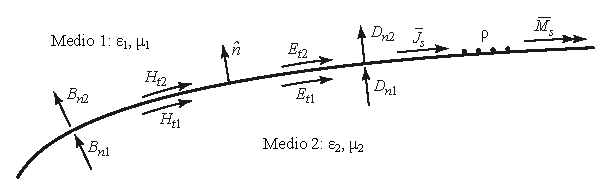
\includegraphics[width=0.8\textwidth]{intro_electro/condiciones_borde.eps}
	\caption{Corrientes, campos y carga superficial en una interfaz general entre dos medios \cite{Pozar:MwEngineering}}
	\label{fig:condiciones_borde}
\end{figure}

Si se considera una interfaz entre dos medios, como la que se muestra en la figura \ref{fig:condiciones_borde}, a partir de las ecuaciones de Maxwell y los teoremas integrales, se pueden deducir las siguientes condiciones de borde:
\begin{subequations}
	\label{eq:condiciones_borde}
	\begin{align}
		\hat{n} \cdot (\vec{D}_{2} - \vec{D}_{1}) & = \rho_s \\
		\hat{n} \cdot (\vec{B}_{2} - \vec{B}_{2}) & = 0 \\
		\hat{n} \times (\vec{E}_2 - \vec{E}_1)  & = - \vec{M}_s \\
		\hat{n} \times (\vec{H}_2 - \vec{H}_1) & = \vec{J}_s
	\end{align}
\end{subequations}

\subsubsection{Campos sobre una superficie dieléctrica}
Dado que en una interfaz entre dos dieléctricos no hay carga eléctrica ni densidades de corriente, las ecuaciones \ref{eq:condiciones_borde} establecen que las componentes normales de los vectores $\vec{D}$ y $\vec{B}$ se conservan, y que las componentes tangenciales de $\vec{E}$ y $\vec{H}$ también lo hacen.

\subsubsection{Campos sobre una superficie conductora eléctrica}
Si el conductor no tiene pérdidas ($\sigma \rightarrow \infty$), todos los campos deben ser cero en su interior, dado que la profundidad de penetración se anula. Considerando, además, que $\vec{M}_s = 0$, la componente tangencial del campo eléctrico, $E_t$ desaparece sobre la superficie del conductor. Dado que la diferencia entre las componentes normales del campo magnético está dada por $\vec{J}_s$, y el campo magnético debe anularse en el conductor, la densidad de corriente superficial está dada únicamente por el campo magnético externo al conductor. En el mismo sentido, la densidad de carga superficial $\rho_s$ es la expresión, sobre la superficie del conductor, de la componente normal de $\vec{D}$.

% SKIN DEPTH

\subsubsection{Campos sobre una superficie conductora magnética}
Dado que la superficie conductora magnética representa el caso dual al de la superficie conductora eléctrica, en este caso se espera que la componente tangencial de $\vec{H}$ se anule sobre la superficie, mientras que la componente tangencial del campo eléctrico dé lugar a corrientes magnéticas sobre la misma.

%%%%% QUEDA DECRI QUE PASA CON UNA CORRIWENTE EN HORIZRAON O VERTICAL - LIBRO DE YAMAT, PAG 10.
%% COMPLETAR CON COLLIN %%

\section{Ecuación de onda}
\label{subsec_eq_de_onda}
%%%%

Al considerar una región del espacio lineal, isotrópica y homogénea, se puede calcular el rotor de la primera ecuación de Maxwell, aplicar la segunda ecuación y, recordando que $\nabla \times \nabla \times \vec{E} = \nabla \nabla \cdot \vec{E} - \nabla^2\vec{E}$, donde $\nabla \times \vec{E} = \rho/\epsilon$, se puede deducir que:

\begin{align}
	\nabla \times \nabla \times \vec{E} & = -j \omega \mu \nabla \times \vec{H} - \nabla \times \vec{M} \notag \\
	\nabla \nabla \cdot \vec{E} - \nabla^2 \vec{E} & = -j \omega \mu \nabla \times \vec{H} - \nabla \times \vec{M} \notag \\
	\frac{\nabla \rho}{\epsilon} - \nabla^2 \vec{E} & = \omega^2 \mu \epsilon \vec{E} - j \omega \mu \vec{J} - \nabla \times \vec{M} \notag\\
	\nabla^2 \vec{E} + \omega^2 \mu \epsilon \vec{E} & = j \omega \mu \vec{J} + \frac{\nabla \rho}{\epsilon} + \nabla \times \vec{M}
	\label{eq:eq_ondas_completa_E}
\end{align}

en el mismo sentido, para el campo magnético:
\begin{align}
	\nabla \times \nabla \times \vec{H} & = j \omega \nabla \times \vec{D} +  \nabla \times \vec{J} \notag \\
	\nabla \nabla \cdot \vec{H} - \nabla^2 \vec{H} & = j \omega \epsilon \nabla \times \vec{E} + \nabla \times \vec{J} \notag \\
	\frac{1}{\mu} \nabla (\cancelto{0}{\nabla \cdot \vec{B}}) - \nabla^2 \vec{H} & = j \omega \epsilon (-j \omega \vec{B} - \vec{M}) + \nabla \times \vec{J} \notag \\
	\nabla^2 \vec{H} + \omega^2 \epsilon \mu \vec{H} & =  j \omega \epsilon \vec{M} - \nabla \times \vec{J}
	\label{eq:eq_ondas_completa_H}
\end{align}

De las ecuaciones anteriores se observa que el campo magnético está determinado por la componente rotacional de la corriente eléctrica, mientras que el campo eléctrico está determinado por todas las componentes de la misma. De manera análoga, se cumple la relación inversa para el caso de la corriente magnética.

Si, además, la región del espacio es libre de fuentes, se deducen las ecuaciones de Helmholtz para ambos campos, donde $k$ es la constante de propagación o número de onda, en unidades de $(1/m)$:

\begin{subequations}
	\label{eq:Helmholtz}
	\begin{align}
		\nabla \times \vec{E} + k^2 \vec{E} = 0 \label{eq:Helmholtz_E} \\
		\nabla \times \vec{H} + k^2 \vec{H} = 0 \label{eq:Helmholtz_H}
	\end{align}
\end{subequations}
%%%%

Para el caso sin pérdidas se puede expresar como $k = \omega \sqrt{\mu \epsilon}$, mientras que si se considera que existen pérdidas óhmicas, las mismas pueden ser tenidas en cuenta si $k$ asume el valor complejo $-j\gamma$, con $\gamma = j\alpha + \beta = j \omega \sqrt{\mu \epsilon} \sqrt{1-j \sigma/(\omega \epsilon)}$. Para el caso de un buen conductor, $\gamma = j\alpha + \beta = j \omega \sqrt{\mu \epsilon} \sqrt{\sigma/(\omega \epsilon)} = (1+j) \sqrt{\omega \mu \sigma/2}$, lo que nos permite definir la profundidad de penetración como $\delta_s = 1/\alpha = \sqrt{2/(\omega \mu \sigma)}$, que decrece con la frecuencia.

En coordenadas cartesianas, la ecuación \ref{eq:Helmholtz_E} se puede escribir como indica la ecuación \ref{eq:Helmholtz_cartesianas_completo}, que además se cumple para todas las coordenadas en que se desarrolla el campo $\vec{E}$. Para cada una de estas coordenadas, resulta sencillo aplicar el método de separación de variables, de forma que $E_i = f(x)g(y)h(z)$ para $i=x, y,$ o $z$, donde las funciones $f(x)$, $g(y)$ y $h(z)$ son independientes.

\begin{equation}
	\label{eq:Helmholtz_cartesianas_completo}
	\nabla^2 \vec{E} + k_0^2 \vec{E} = \frac{\partial^2 \vec{E}}{\partial x^2} + \frac{\partial^2 \vec{E}}{\partial y^2} + \frac{\partial^2 \vec{E}}{\partial z^2} +  k_0^2 \vec{E} = 0
\end{equation}

Sustituyendo, para la ecuación de Helmholtz de cada coordenada, la expresión de $E_i$, se obtiene:

\begin{equation}
	\frac{f''(x)}{f(x)} + \frac{g''(y)}{g(y)} + \frac{h''(z)}{h(z)} + k_0^2 = 0
\end{equation}

Dado que las funciones propuestas son independientes, cada uno de los términos de la ecuación anterior deben dar lugar a una constante:

\begin{equation}
	\frac{f''(x)}{f(x)} = -k_x^2; \qquad \frac{g''(y)}{g(y)} = -k_y^2; \qquad \frac{h''(z)}{h(z)} = -k_z^2
\end{equation}

de manera que:

\begin{equation}
	\label{eq:numero_de_onda}
	k_x^2 + k_y^2 + k_z^2 = k_0^2 \\
\end{equation}

Quedan, entonces, tres ecuaciones diferenciales ordinarias:

\begin{equation}
	\frac{d^2 f}{dx^2} + k_x^2 f = 0; \qquad \frac{d^2 g}{dy^2} + k_y^2 g = 0; \qquad \frac{d^2 h}{dz^2} + k_z^2 h = 0;
\end{equation}

cuyas soluciones son de la forma $e^{\pm j k_i i}$, con $i = x, y$ o $z$, respectivamente. Las soluciones con un signo positivo en el exponente corresponden a ondas que viajan en la dirección negativa ($-x, -y, -z$), mientras que las que tienen un signo negativo corresponden a ondas que viajan en la dirección positiva. Dado que ambas soluciones son válidas y posibles, en función de las condiciones de borde, en general la expresión de un campo $E_i (x, y, z), i=x,y,z$ quedará establecida como la suma de ambas, afectadas por un factor de amplitud dependiente de la coordenada evaluada. Para el caso de ondas que viajan en la dirección positiva:

\begin{equation}
	E_i(x,y,z) = A_i \;e^{-j(k_x x + k_y y + k_z z)}, \quad i=x,y,z
\end{equation}

Lo que indica que la coordenada $i$-ésima del campo eléctrico tendrá un comportamiento exponencial complejo respecto de la posición. 

Si definimos como $\hat{n}$ al versor en la dirección de propagación, podemos definir el vector de número de onda, $\vec{k}$, como:

\begin{equation}
	\label{eq:vector_numero_de_onda}
	\vec{k} = k_x \hat{x} + k_y \hat{y} + k_z \hat{z} = k_o \hat{n}
\end{equation}

De esta forma, se puede expresar, estableciendo $\vec{E}_0 = A \hat{x} + B \hat{y} + C \hat{z}$, y $\vec{r} = x \hat{x} + y \hat{y} + z \hat{z}$, el campo eléctrico como:

\begin{equation}
	\label{eq:electric_field_wave_solution}
	\vec{E} = \vec{E}_0 e^{-j\vec{k} \cdot \vec{r}}
\end{equation}

Para el caso con pérdidas, y considerando que la dirección de propagación es $z$, las componentes $x$ e $y$ se comportan como:

\begin{equation}
E_i(z) = E_i \; e^{-\gamma z} = E_i \; e^{-\alpha z} \; e^{-j \beta z}, \quad i=x,y
\end{equation}

Al expresar la divergencia del campo eléctrico de la ecuación \ref{eq:electric_field_wave_solution}, que en una región sin fuentes es nula, y recordando que $\nabla \cdot (f \vec{A}) = \vec{A} \cdot \nabla f + f \nabla \cdot \vec{A}$, se obtiene:

\begin{align}
	\nabla \cdot \vec{E} = \nabla \cdot \vec{E}_0 e^{-j\vec{k} \cdot \vec{r}} & = \vec{E}_0 \cdot \nabla e^{-j \vec{k} \vec{r}} + e^{-j \vec{k} \vec{r}} \cancelto{0}{\nabla \cdot \vec{E}_0} = 0 \\
	& -j \vec{k} \cdot \vec{E}_0 e^{-j \vec{k} \vec{r}} = 0
\end{align}

De lo que se puede deducir que $\vec{k} \cdot \vec{E}_0 = 0$, de modo que el campo eléctrico, en una onda plana, es siempre perpendicular a la dirección de propagación.

De la ecuación de Faraday (\ref{eq:Faraday_harmonic}), considerando espacio libre de cargas, se puede deducir que el campo magnético es siempre ortogonal al campo eléctrico y a la dirección de propagación, y que los campos están relacionados de forma que \cite{Fernandez:Electromag}:

\begin{equation}
	\vec{H}(\vec{r},t) = \pm \frac{\hat{n} \times \vec{E}(\vec{r},r)}{\eta}
\end{equation}

donde $\eta$ es la impedancia de onda, que tiene la forma $\eta = j \omega \mu / \gamma$. Para el caso del vacío, la impedancia intrínseca se denota $\eta_0$ y tiene un valor de $377\; \Omega$, mientras que para otros materiales está determinada por su permitividad eléctrica y permeabilidad magnética, y puede ser compleja si hay pérdidas.

La velocidad de fase se define como $v_p=\omega/\beta$, que para el caso sin pérdidas queda como $1/\sqrt{\mu \epsilon}$, y que para el caso particular del vacío, se expresa como $1/\sqrt{\mu_0 \epsilon_0} = c$, donde $c$ es la velocidad de la luz en el vacío. Así, la velocidad de fase en cualquier medio material sin pérdidas resulta $c/\sqrt{\epsilon_r \mu_r}$.

La longitud de onda, $\lambda$, es la distancia espacial entre dos máximos sucesivos, por lo que se expresa como $\lambda = 2\pi / k = v_p/f$.

\subsection{Incidencia normal de una onda plana sobre una interfaz}


\subsection{Incidencia oblicua de una onda plana sobre una interfaz}

\section{Guias de ondas}
\label{subsec_guias_de_ondas}
%%%%
LOREM IPSUM
%Pozar, pag 171
%%%%

\subsection{Guía de ondas dieléctricas con plano de tierra}




\section{Líneas de transmisión}
\label{subsec_lineas_de_transmision}
%%%%
LOREM IPSUM
% Venkateswaran, cap 1.
%%%%
\section{Antenas}
\label{subsec_antenas}
%%%%
LOREM IPSUM
%%%%
\subsection{Regiones de campo}
\label{subsubsec_regiones_de_campo}
%%%%
LOREM IPSUM
%%%%
\subsection{Diagramas de radiación}
\label{subsubsec_diag_de_rad}
%%%%
LOREM IPSUM
%%%%
\subsection{Potencia total radiada e intensidad de radiación}
\label{subsubsec_pot_total_radiada}
%%%%
LOREM IPSUM
%%%%
\subsection{Directividad, eficiencia y ganancia}
\label{subsubsec_directividad}
%%%%
LOREM IPSUM
%%%%
\subsection{Polarización}
\label{subsubsec_polarizacion}
%%%%
LOREM IPSUM
%%%%

\subsection{Impedancia de entrada}
\label{subsec_imp_entrada}
%%%%
LOREM IPSUM
%%%%
\subsection{Acoplamiento mutuo}
\label{subsec_acoplamiento}
%%%%
LOREM IPSUM
%%%%
\subsection{Dieléctricos y pérdidas dieléctricas}
\label{subsec_dielectricos}
%%%%
LOREM IPSUM
% LibroSinNombre, pagina 816
%%%%
\subsection{Parámetros S}
\label{subsec_parametros_s}
%%%%
LOREM IPSUM
% Pozar, pag 178
%%%%

\subsection{Antenas Microstrip}
\label{subsec_antenas_microstrip}
%%%%
LOREM IPSUM
%%%%
\subsubsection{Modelo de líneas de transmisión}
\label{subsubsec_microstrip_modeloLineas}
%%%%
LOREM IPSUM
% LibroSinNombre, pahgina 534
%%%%
\subsubsection{Modelo de cavidades multimodo}
\label{subsubsec_microstrip_modeloCavidades}
%%%%
LOREM IPSUM
% Pozar, rezonadores, capitulo 6
%%%%

\subsection{Acoplamiento mutuo en antenas Microstrip}
\label{subsec_acoplamiento_microstrip}
%%%%
LOREM IPSUM
%%%%
% LibroSinNombre, pagina 562 y 631
\subsubsection{Ondas de superficie}
\label{subsubsec_microstrip_ondas_superficie}
%%%%
LOREM IPSUM
%%%%
% Engheta, pagina 289
% Rahim (tesis), pagina 28
% Collin, capitulo de Surface waveguides, pag 697
% Paper de Barlow.
% Pozar, pag 138
% Tesis de Kovacs, pagina 8
% Tesis de Zheng, apendice A, pag 48. Interfaces con diel y con metales.

